\documentclass{beamer}

\usepackage{animate}
\usepackage{subfigure}
\usetheme{AnnArbor}
\usecolortheme{beaver}


\title 
{Feature Extraction and Classification of Plankton}
\subtitle
{ We done things }
\author{Dane Skinner \and Nick Hockensmith \and Kevin Park}
\institute
{Oregon State University}
\date
{May 15, 2014}
\begin{document}

%----------------------------------
% FRAME 2
%----------------------------------
\begin{frame}
\frametitle{Outline}
	\begin{itemize}
	\item Brief Introduction
	\item Feature Extraction
	\item Classification Models: Random Forest \& kNN 
	\item Conclusion and Final Thoughts
	\end{itemize}
\end{frame}
%----------------------------------
% FRAME 3
%----------------------------------
\begin{frame}
\frametitle{Introduction}
\begin{itemize}
\item We looked at tiny little things
\end{itemize}

\end{frame}

%----------------------------------
% FRAME 4
%----------------------------------

\begin{frame}
\frametitle{Questions of Interest}
\end{frame}

%----------------------------------
% FRAME 5
%----------------------------------

\begin{frame}
\frametitle{Kratuchok's Moments}
$\bullet$ Calculating \textit{Kratuchok's} moments,
\begin{equation*}
Q_{nm} = \sum_{x=0}^{N-1}\sum_{y=0}^{M-1}\bar{K}_n(x;p_1,N-1)\bar{K}_m(y;p_2,M-1)f(x,y),
\end{equation*}
where  $f(x,y)$ is the pixel intensity and ($K_n(a;p,N$) are the weighted Krawtchouk polynomials, and $n\in \mathbb{N}$ is order of the moment in the x- or y-direction.\\
$\bullet$ Kratuchok moments are invariant under scaling, rotation, and translation. \\
\end{frame}

%----------------------------------------------------------------
% FRAME 5.5
%----------------------------------------------------------------

%----------------------------------
% FRAME 6
%----------------------------------

\begin{frame}
\frametitle{Histogram Method}
$\bullet$ Some of species of plankton give distinct distributions of gray scale values. 
\begin{center}
	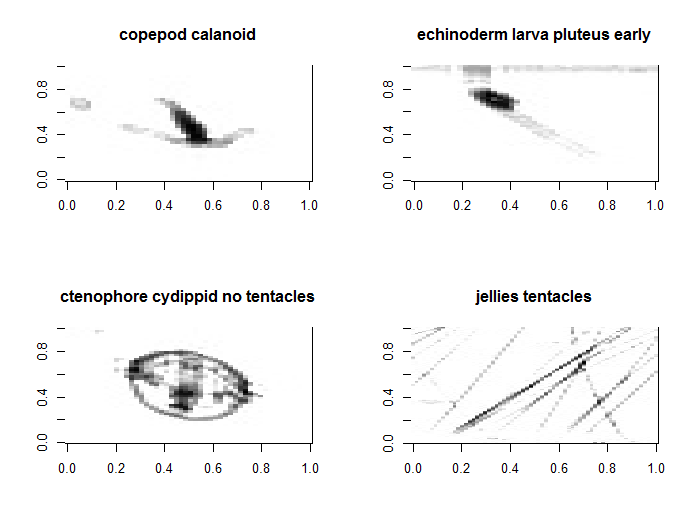
\includegraphics[scale=0.23]{images.png}
	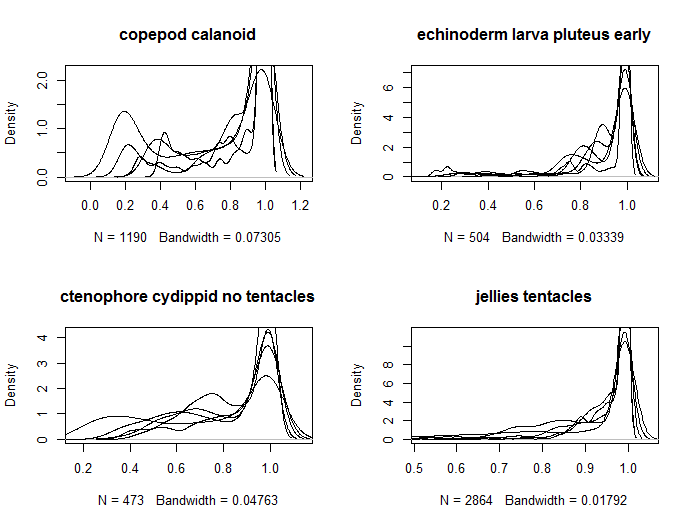
\includegraphics[scale=0.23]{grayscale.png}
\end{center}
\end{frame}

\begin{frame}
	\frametitle{Histogram Method}
	$\bullet$ The grayscale is on a [0,1] interval and we partition the interval into a width of 0.1.\\
	$\bullet$ We have count the number of values that are between $[0,0.1],[0.1,0.2],\cdots, [0.9,1]$.\\ 
	\begin{center}
		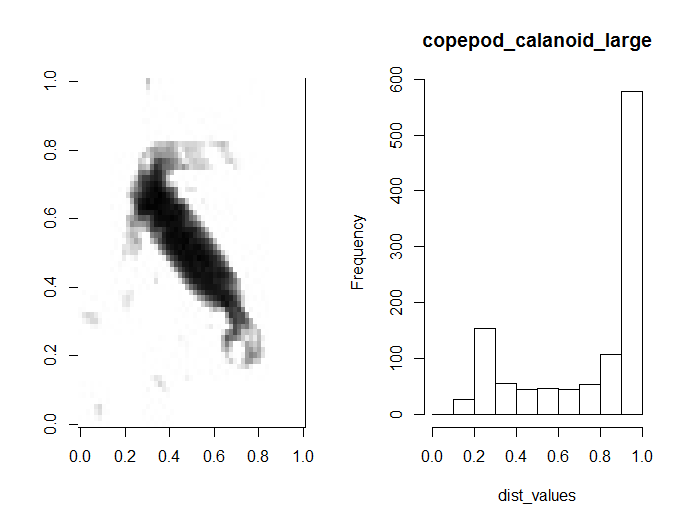
\includegraphics[scale=0.3]{bin_method.png}
	\end{center}
\end{frame}
%----------------------------------
% FRAME 7
%----------------------------------
\begin{frame}
\frametitle{Indicio Package and kNN}
$\bullet$ This produces a sparse, 2048 digit feature vector for each image that can then be used to calculate the Euclidean distances between different feature vectors
\end{frame}

%----------------------------------------------------------------
% FRAME 8
%----------------------------------------------------------------

\begin{frame}
	\frametitle{Kaggle Results:}
$\bullet$ We are surprised as much as you.\\
$\bullet$ Histogram method produced a score of 3.29. \\
\begin{center}
	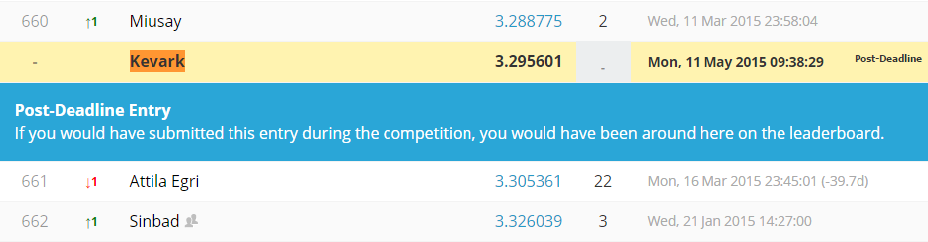
\includegraphics[scale=0.3]{submission.png}
\end{center}
$\bullet$ Combination of Histogram and Moments produced a score of 2.66. \\
\begin{center}
	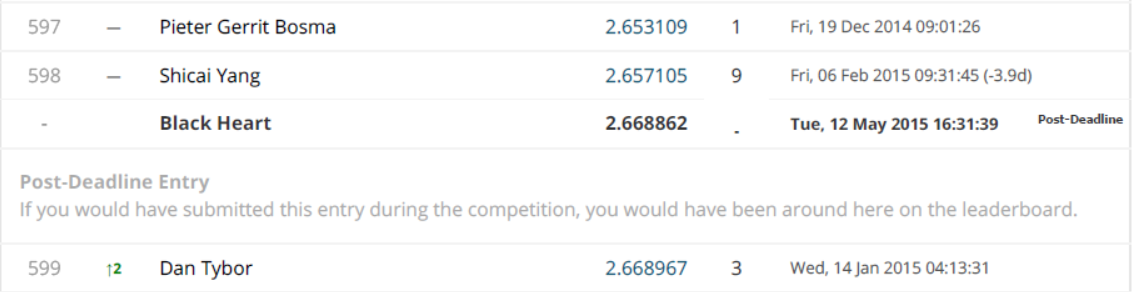
\includegraphics[scale=0.25]{combined.png}
\end{center}
\end{frame}

%----------------------------------------------------------------
% FRAME 9 
%---------------------------------------------------------------

\begin{frame}
	\frametitle{Conclusions and Final Thoughts}
	\begin{itemize}
		\item Apply image processing algorithms 
	\end{itemize}
\end{frame}


\end{document}
